\title{EE 385V - Brain Computer Interaction Homework 1 Report}
\author{Thomas Plantin \\ }
\date{\today}

\documentclass[12pt]{article}

\usepackage[export]{adjustbox}

\usepackage{xcolor}
\pagecolor{white}

\usepackage{graphicx}
\graphicspath{ {./images/} }

\newcommand\tab[1][0.60cm]{\hspace*{#1}}

\begin{document}
\maketitle

%%%%%%%%%%%%%%%%%%%%%%%%%%%%%%
\section{How does the dataset look like?}
\subsection{What do these dimensions mean?}
The signal is the recorded EEG signal at a sampling frequency of 250-Hz, and the triggers represent recording interval.

%%%%%%%%%%%%%%%%%%%%%%%%%%%%%%
\section{Triggers}
\subsection{What do the triggers mean in our case?}
In our case, the triggers are starting points of the trials.

\subsection{Can we deduce the number of trials? How?}
Yes, by computing the length of the array ‘trigger’. In our case, the length is 90, so there are 90 triggers.\clearpage

%%%%%%%%%%%%%%%%%%%%%%%%%%%%%%
\section{Raw Signals}
\subsection{Plot the raw signal. On top, plot when the triggers appear.}

\begin{figure}[!htb]
    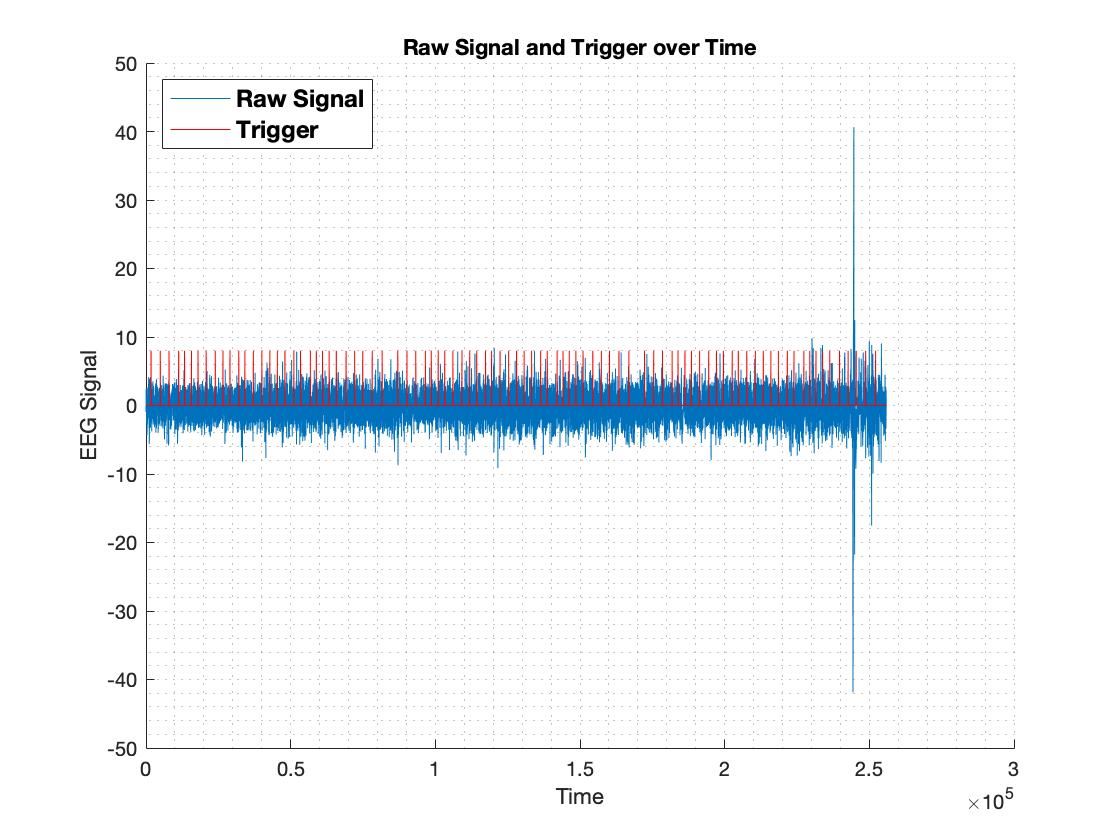
\includegraphics[scale=0.4]{raw_trigger}
\end{figure}

%%%%%%%%%%%%%%%%%%%%%%%%%%%%%%
\section{Filtering}
\subsection{Why filtering data?}
We filter data to mitigate noise and to remove artifacts so that we can observe the relevant behaviors in our signal.\clearpage

\subsection{Filter signal in alpha and beta bands (9-11 Hz and 18-22 Hz, respectively). Then plot the two filtered signals on top of the raw signal.}

\begin{figure}[!htb]
    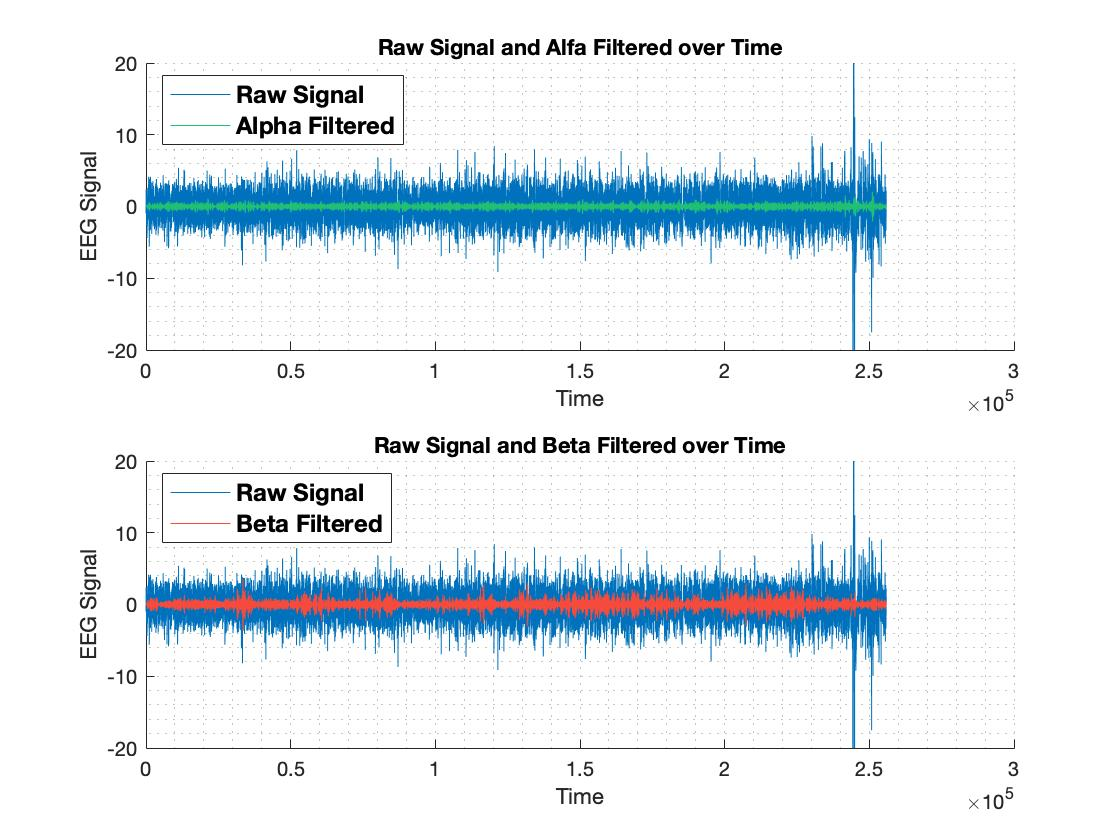
\includegraphics[scale=0.4]{alpha_beta}
\end{figure}\clearpage

%%%%%%%%%%%%%%%%%%%%%%%%%%%%%%
\section{Power and Moving Average}
\subsection{Compute the power of the signal, then plot it on top of the previous signals.}
\begin{figure}[!htb]
    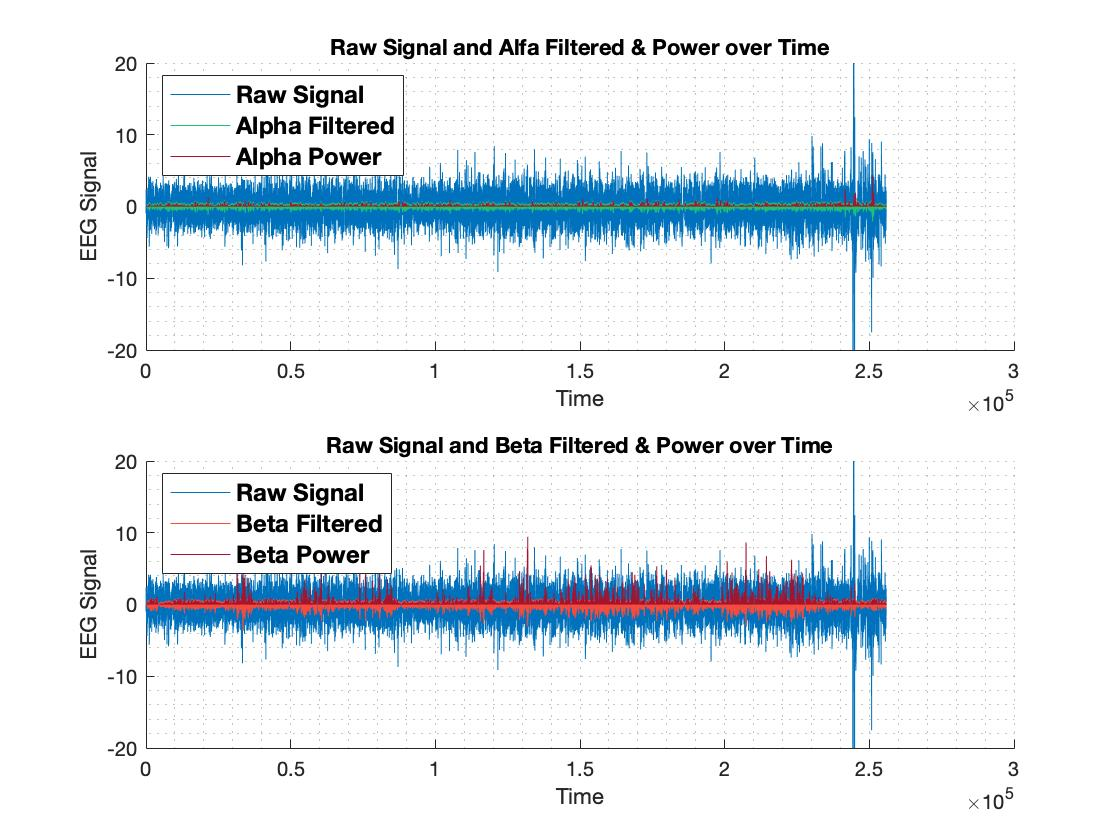
\includegraphics[scale=0.4]{power_1}
\end{figure}

\subsection{What is the moving average? Why apply it?}
It attenuates the effect of outliers on the rest of the data and it suppresses high frequency noise.\clearpage

\subsection{Compute and plot it for alpha and beta band.}
\begin{figure}[!htb]
    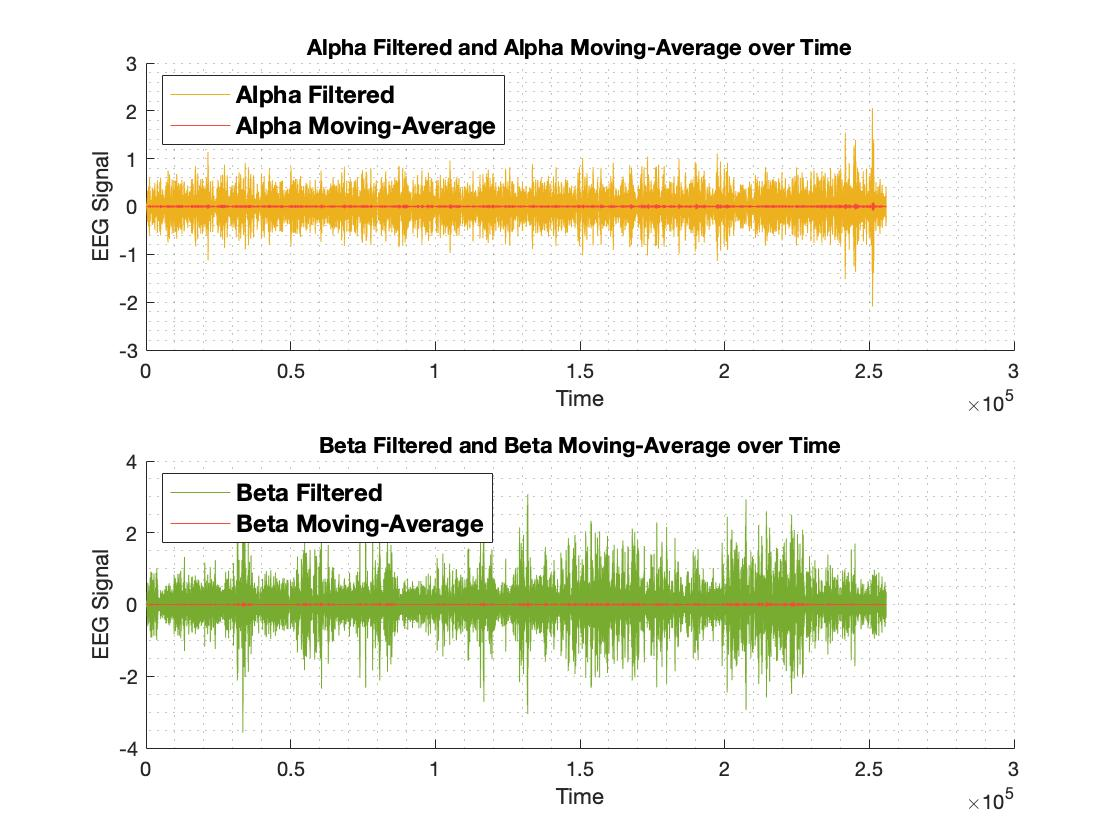
\includegraphics[scale=0.4]{mov_avg}
\end{figure}

\subsection{What happens by changing the window size?}
By increasing the window size, you increase the number of samples that are being averaged. And the more samples are being averaged, the less the value of a given recording has an effect on the overall trend.\clearpage

%%%%%%%%%%%%%%%%%%%%%%%%%%%%%%
\section{Single Trial Plots}
\subsection{Plot some trials of raw signal}
\begin{figure}[!htb]
    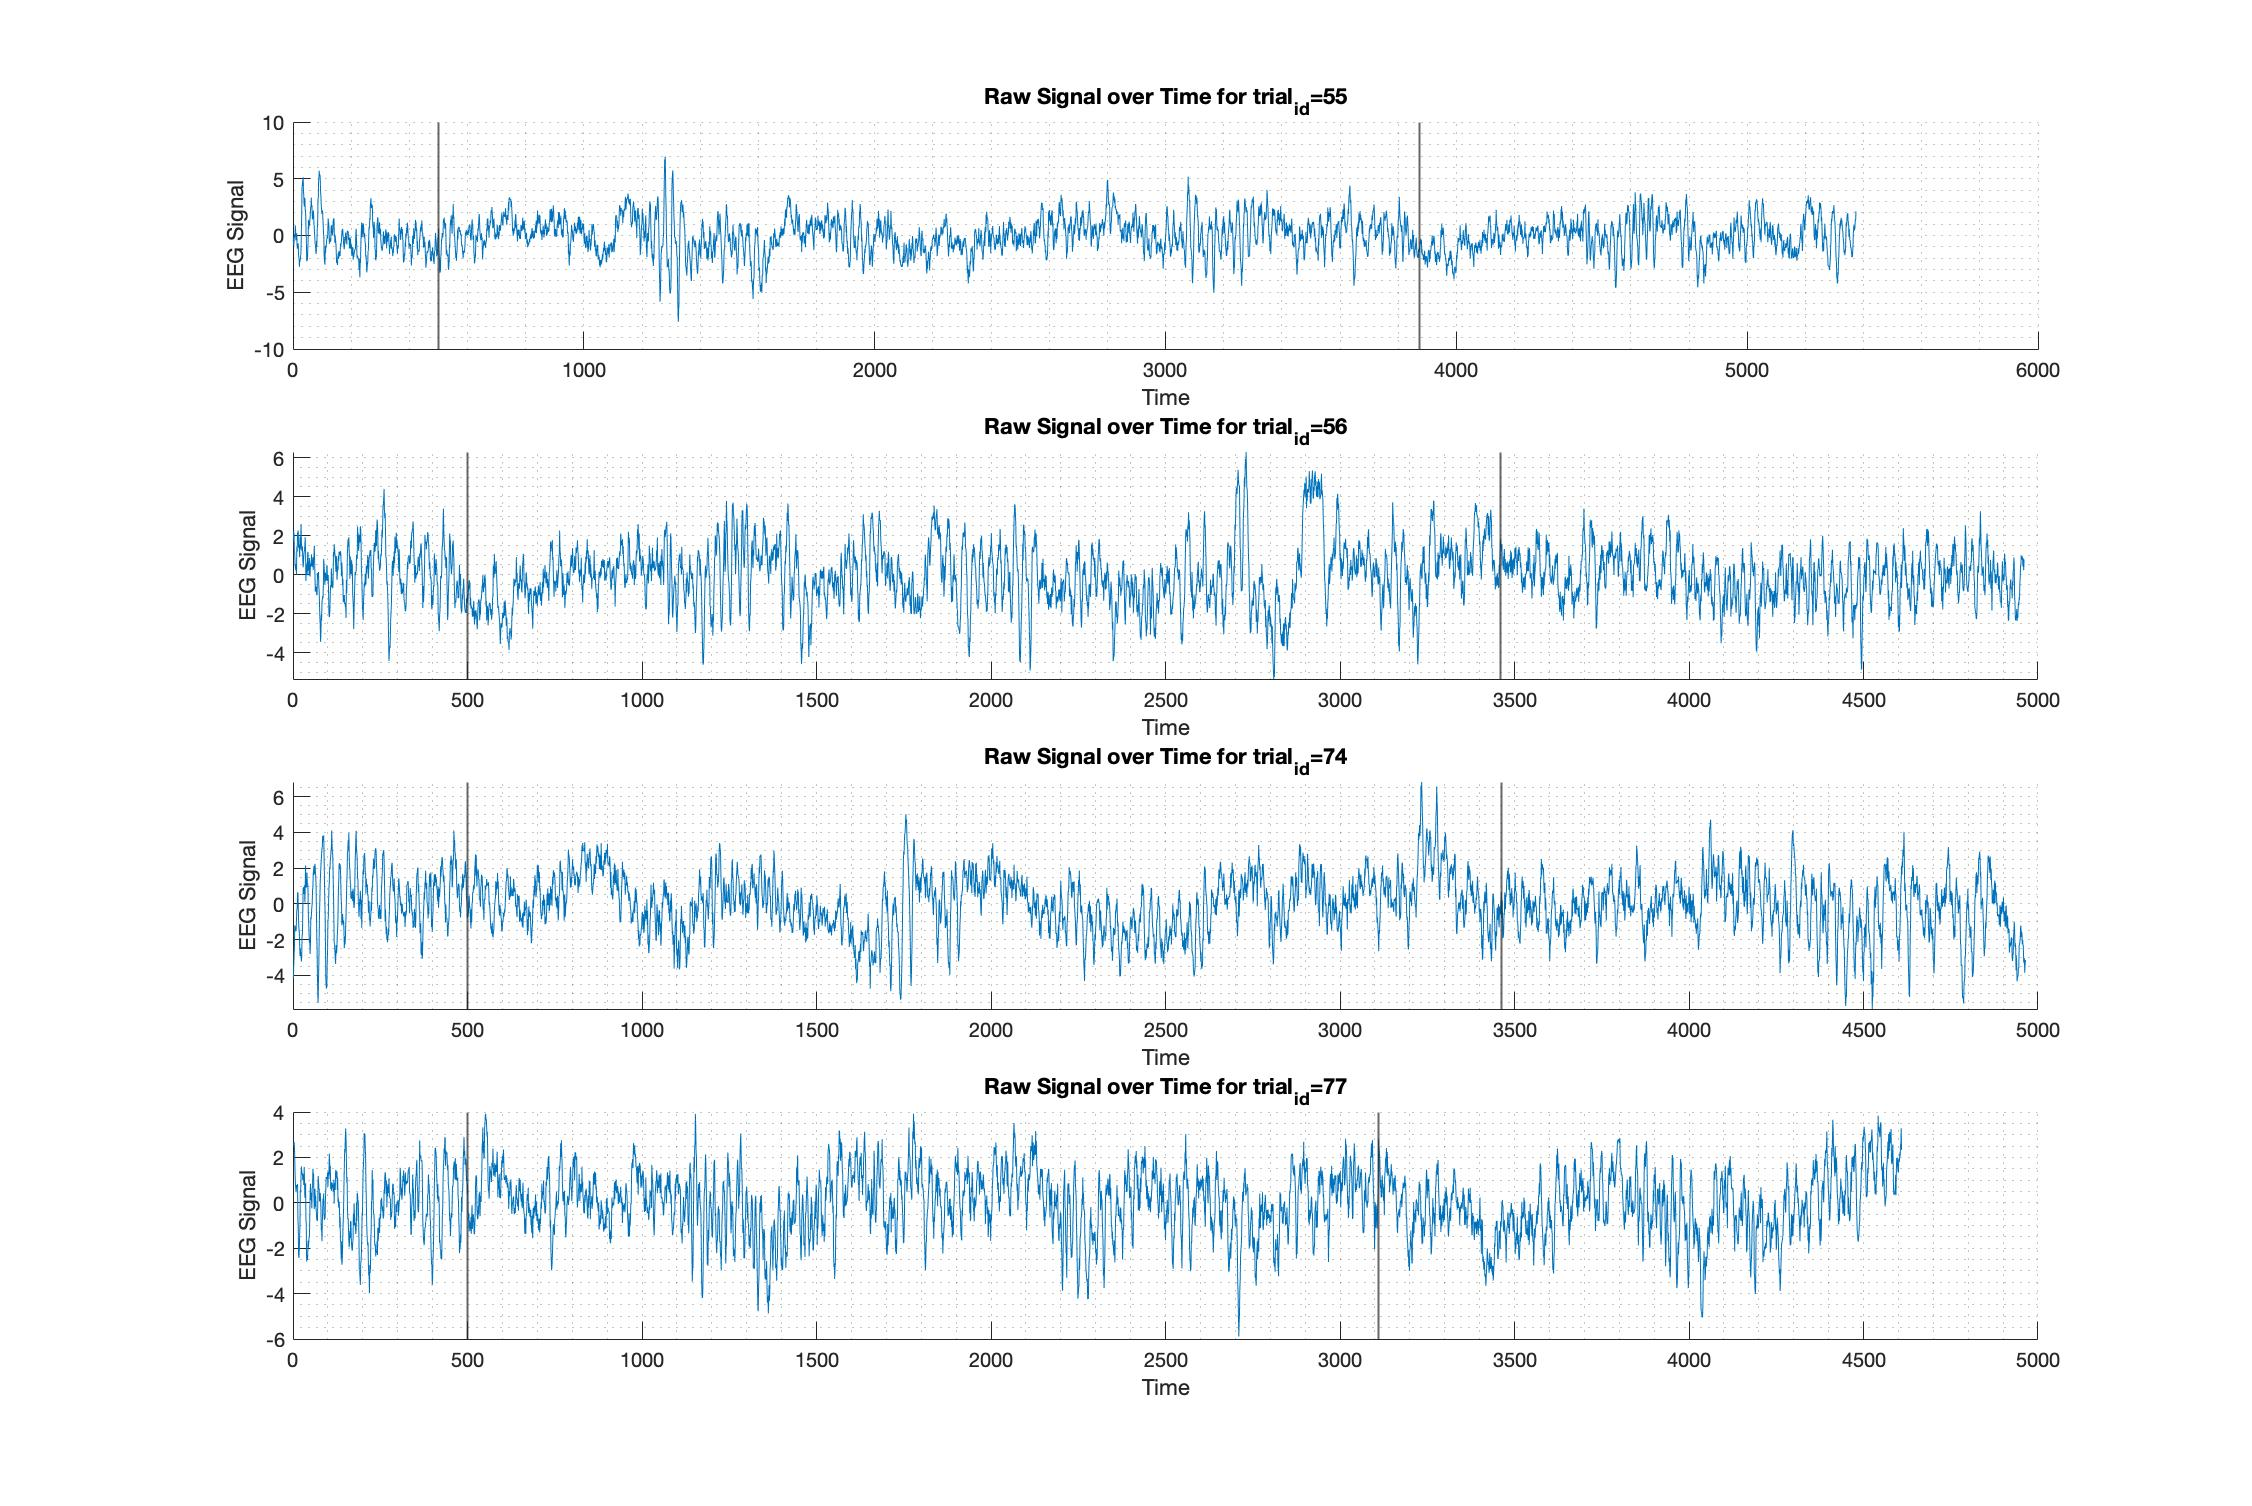
\includegraphics[scale=0.3, center]{raw_trials}
\end{figure}\clearpage

\subsection{Plot the same trials filtered in alpha and beta bands}
\begin{figure}[!htb]
    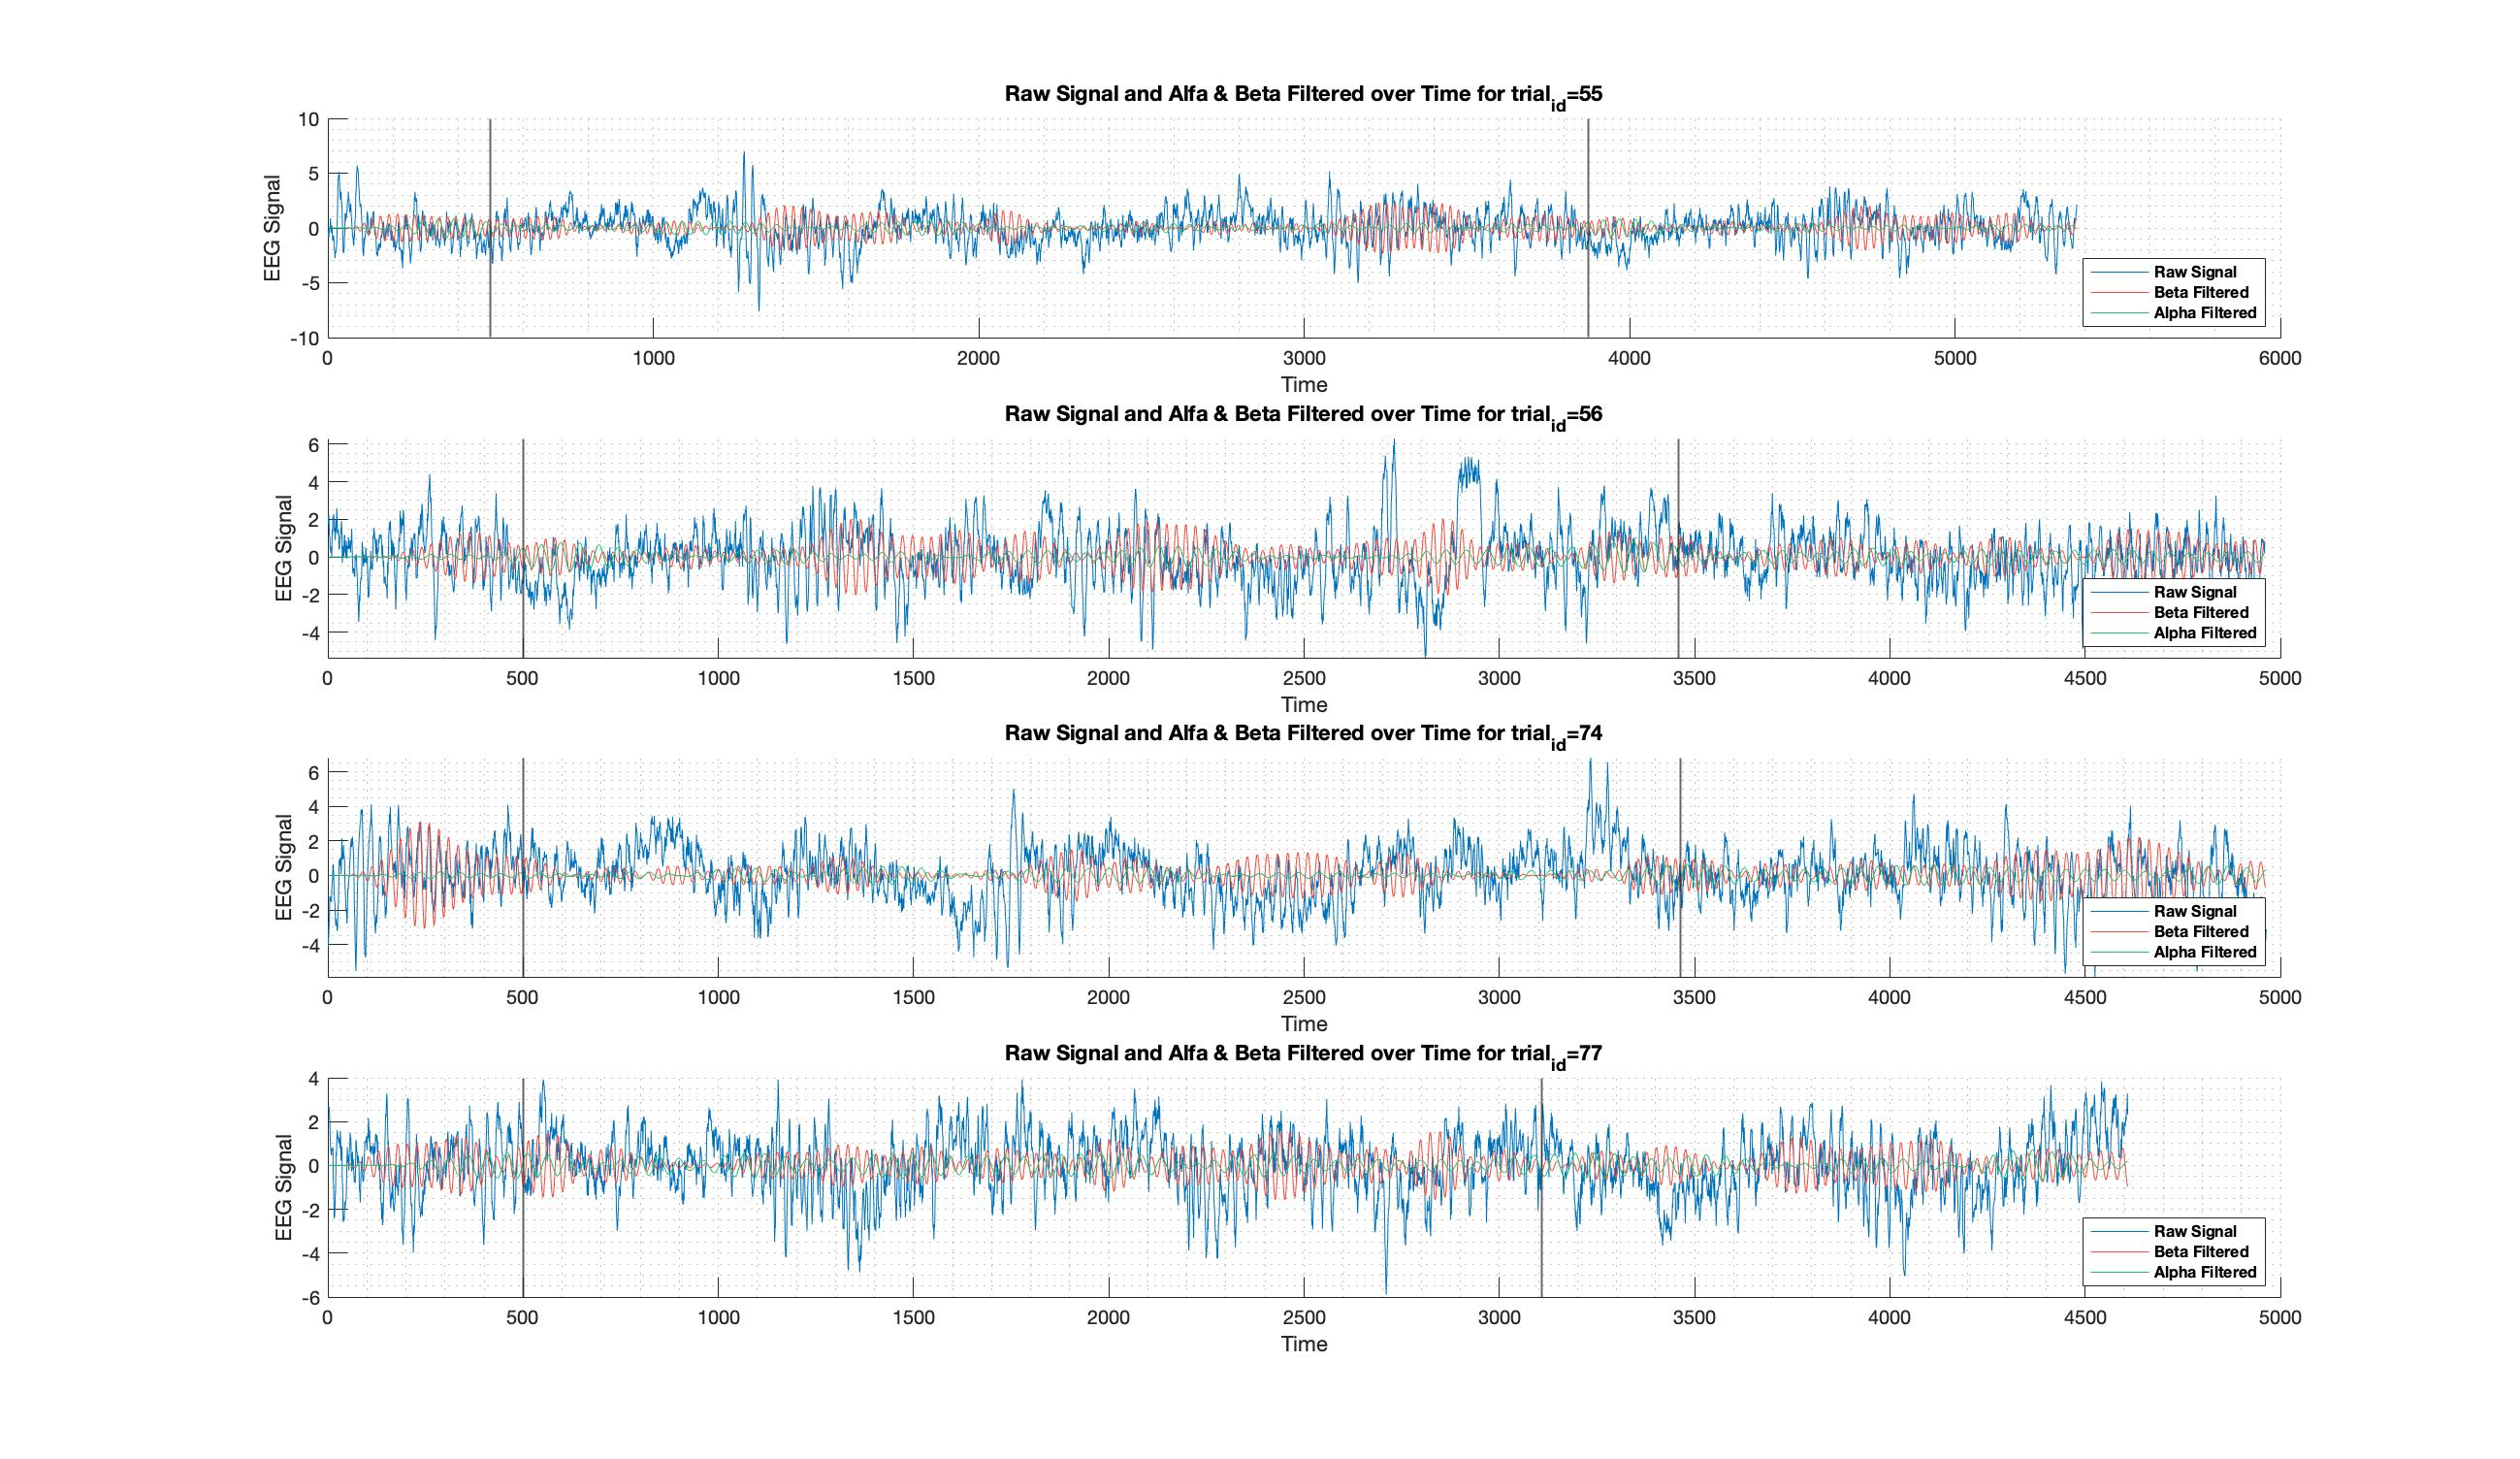
\includegraphics[scale=0.28, center]{alpha_beta_trials}
\end{figure}\clearpage

\subsection{What can you infer from the different plots? Are there (dis)similarities between different bands?}
\tab Similarities:
\begin{itemize}
  \item There is a synchronization before the trigger, then a desynchronization at the trigger, and then a rebound when the action is imagined.
  \item All of the beta filtered signals have larger amplitude than the alpha filtered signals.
\end{itemize}

Dissimilarities:
\begin{itemize}
  \item They have different frequency content.
  \item They have different energy for this task.
\end{itemize}

\subsection{Are there (dis)similarities between trials?}
\tab Similarities:
\begin{itemize}
  \item There is a synchronization before the trigger, then a desynchronization at the trigger, and then a rebound when the action is imagined.
\end{itemize}

Dissimilarities:
\begin{itemize}
  \item The triggers are not evenly spaced out.
\end{itemize}\clearpage

%%%%%%%%%%%%%%%%%%%%%%%%%%%%%%
\section{Grand Average}
\subsection{Plot averaged signals of alpha and beta power.}
\begin{figure}[!htb]
    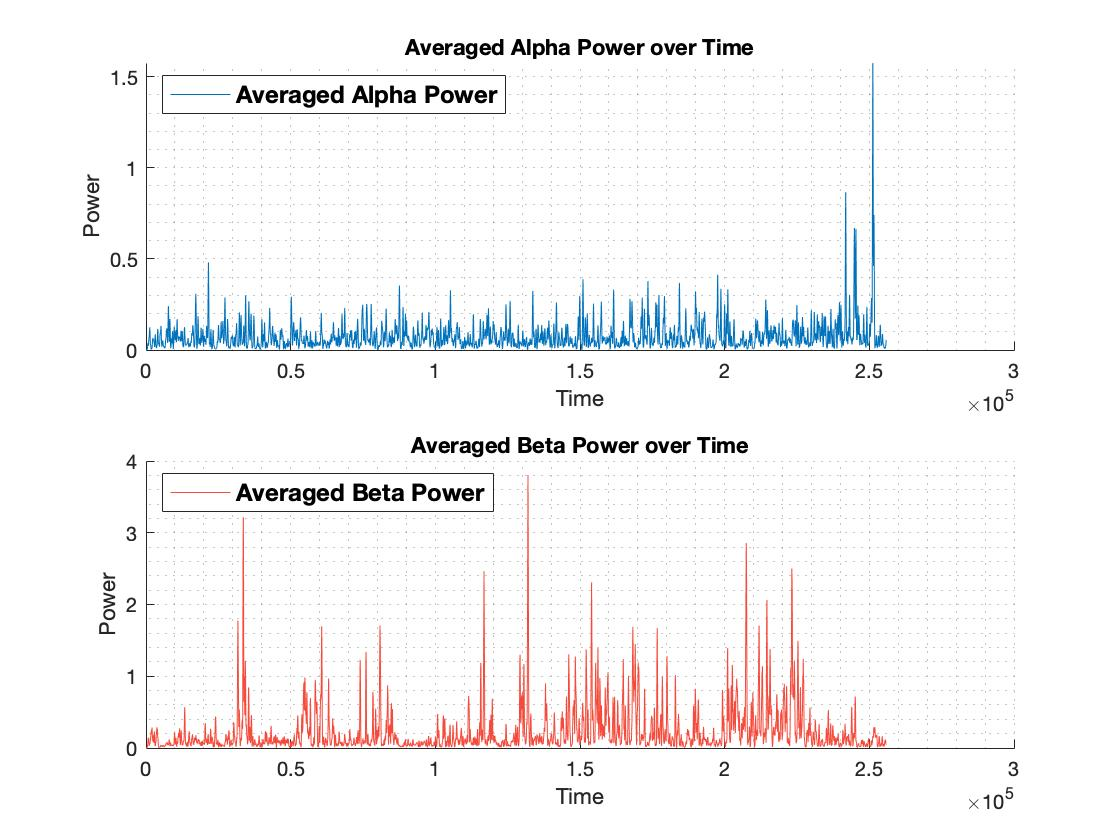
\includegraphics[scale=0.4, center]{alpha_beta_power}
\end{figure}

\subsection{What can we infer from these plots?}
We can see that the averaged alpha signal power is greater than averaged beta signal power.\clearpage

\subsection{What are the differences between single trial and grand average signals?}
They are both useful, but you can’t create a final grand average in real time. So it is best to rely on the single trial and to use a grand average as the fingerprint to check against that single trial.

\subsection{What is more useful for online real time BCI?}
They are both useful, but you can’t create a final grand average in real time. So it is best to rely on the single trial and to use a grand average as the fingerprint to check against that single trial.

\subsection{What are the main difficulties when dealing with single trial analysis?}
\begin{itemize}
  \item Noise
  \item Artifacts
  \item The subject's focus and preparation
  \item More challenging filtering approach
\end{itemize}

\end{document}